\section{Insert-First-Verfahren}
% Was ist das Min Dist Verfahren?
    % Nodes werden in der Reihenfolge ihres Auftretens in den Graphen eingefügt
    % Insert-First = dadurch insert-random  
% Wie funktioniert es
    % Ein neuer Graph mit einem Pfad der länge n wird erzeugt
    % Die Nodes des Pfades des Graphen seien Y1,Y2,Y3,Y4...
    % Die erst Node des Pfads wird mit der ersten Node in der Liste der Verfügbaren Nodes befüllt (= Ausgangs-Node)
    % Die zweite Node wird ebenso aus den verfügbaren Nodes angehängt (ist nun an zweiter Stelle)
    % Nun wird durch die restlichen Verfügbaren Nodes iteriert
    % Node X sei Gegenstand des momentanen Iterationdurchlaufs 
    % Für X wird beginnend mit Y2 die Distanz zwischen Yn-1 und X + Distanz zwischen Yn und X errechnet
    % resultierend aus diesen Berechnungen wird die beste Stelle gesucht, um X in den Pfad einzufügen
% Teile des Quellcodes zeigen

Das Insert-First-Verfahren ist ein heuristischer Lösungsansatz des \ac{TSP}s, bei dem das Betrachten der Knoten zum Aufbau eines Graphen in zufälliger Reihenfolge, bzw. in der Reihenfolge ihrer Erzeugung geschieht.
Dabei wird immer ein Knoten betrachtet und in Abhängigkeit von seiner Entfernung zu den anderen Knoten in den Graphen eingefügt.

\subsection{Funktionsweise}
Zu Beginn des Insert-First-Verfahrens wird ein neuer Graph erzeugt, welcher als Eingabewerte eine Liste von Knoten, hier bezeichnet als \lstinline{nodes}, mit $K_1, K_2,  \ldots ,K_n$ und der Länge $n$ erhält. 
Dadurch wird festgelegt, dass der Graph $n$ Knoten enthalten wird.
Nun wird der $K_1$, der erste Knoten aus der Liste in den Graph an erster Stelle eingefügt. 
Dies geschieht so oder ähnlich bei allen Verfahren, um einen statischen Ausgangspunkt zu gewährleisten und somit vergleichbare Ergebnisse zu erzielen.
Anschließend wird noch der zweite Knoten angehängt.
\begin{lstlisting}[caption={Zuweisung des ersten und zweiten Knotens}]
path[0] = nodes[0];
path[1] = nodes[1];  
\end{lstlisting}
Das Vorgehen für das Einfügen der restlichen Knoten lässt sich wie folgt beschreiben: 
Sei $G$ ein Graph mit übergebener Liste von Knoten  $K_1,\ldots,K_n$ und bereits eingefügten Knoten $K_1,\ldots,K_m$ mit $2 > m < n$, später im Programm als \lstinline{path} bezeichnet. 
Die Knoten, die noch eingefügt werden müssen, werden in der Reihenfolge ihres Auftretens in der übergebenen Liste in den Graphen eingefügt, womit der als nächstes einzufügende Knoten immer $K_{i}$ mit $i = m + 1$ ist.
\\
Um die Stelle zu ermitteln, in die $K_i$ eingefügt werden soll, müssen die Distanzen zu Vorgänger und Nachfolger berechnet und die geringste Entfernung ermittelt werden. 
Hierzu wird durch die Knoten beginnend mit $K_2$ bis $K_{m+1}$ iteriert. Dabei sei $K_j$ der Knoten des aktuellen Iterationdurchlaufs. 
Nun wird die Distanz zwischen $K_{j-1}$ und $K_i$ mit der Distanz zwischen  $K_{j}$ und $K_i$ addiert. Hierbei muss beachtet werden, dass bei der Betrachtung von $K_{j=m+1}$ keine wirkliche Distanz zu $K_i$ errechnet werden kann, da nur $m$ Knoten im Graphen sind. Stattdessen wird angenommen, dass die Distanz 0 beträgt, sodass ein Anfügen an das Ende des Graphen simuliert wird.
\\
In Java Quellcode bedeutet dies konkret:
\begin{lstlisting}[caption={Ermittlung der Distanzen}, label={lst:distjava}]
double currentDistance = 
    ((path[j] != null) ? distances.getDistanceById(path[j], nodes[i]) : 0)
    + distances.getDistanceById(path[j - 1], nodes[i]);

\end{lstlisting}
Das niedrigste Ergebnis von \lstinline{currentDistance} wird zusammen mit dem dazugehörigen Index vermerkt. Nachdem die niedrigste Distanz für $K_i$ errechnet wurde kann anhand des Index' der Knoten an der besten Stelle in den Graphen eingefügt werden. 
Einfügen bedeutet hier, dass alle Knoten, deren Index gleich oder höher dem niedrigsten Index für $K_i$ ist nach hinten verschoben werden. Nachdem alle Knoten auf diese Weise nach hinten verschoben wurden, kann $K_i$ an die Stelle des niedrigsten Index eingefügt werden, ohne, dass andere Knoten verloren gehen.
\begin{lstlisting}[caption={Einfügen von Knoten in einen bestehenden Graph}, label={lst:mergeIntojava}]
private static Node[] mergeNodeIntoGraph(Node[] path, Node node, int index) {
    for (int i = path.length - 2; i >= index; i--) {
        path[i + 1] = path[i];
    }
    path[index] = node;
    return path;
}
\end{lstlisting}
Beispielhaft sähe das mit den vorher festgelegten Bezeichnungen wie folgt aus: 
\begin{addmargin}[1em]{2em}
\lstinline{path = } $K_1, K_2, K_4, K_3$ und $K_{i = 5}$ 
\end{addmargin}
Durch das ermitteln der Distanzen zu den bereits eingefügten Knoten wird bekannt, dass $K_i$ am besten zwischen $K_4$ und $K_3$ eingefügt werden soll, also der Index $4$ vermerkt wird. Durch das Einfügen nach \vref{code:mergeIntojava} entsteht folgender Pfad:
\begin{addmargin}[1em]{2em}
\lstinline{path = } $K_1, K_2, K_4, K_5, K_3$
\end{addmargin}
für den Graphen.

\subsection{Ergebnisse und Schwächen}
Bei dem Einsatz des oben beschriebenen Algorithmus kommt es Ergebnissen, die in ihrer Qualität nah an die optimale Lösung herankommen, teilweise aber auch weit von ihr abweichen können.

    

\begin{figure}[!ht]
    \begin{center}
    \subfloat[$m = 2$\label{subfig-1:m2}]{%
      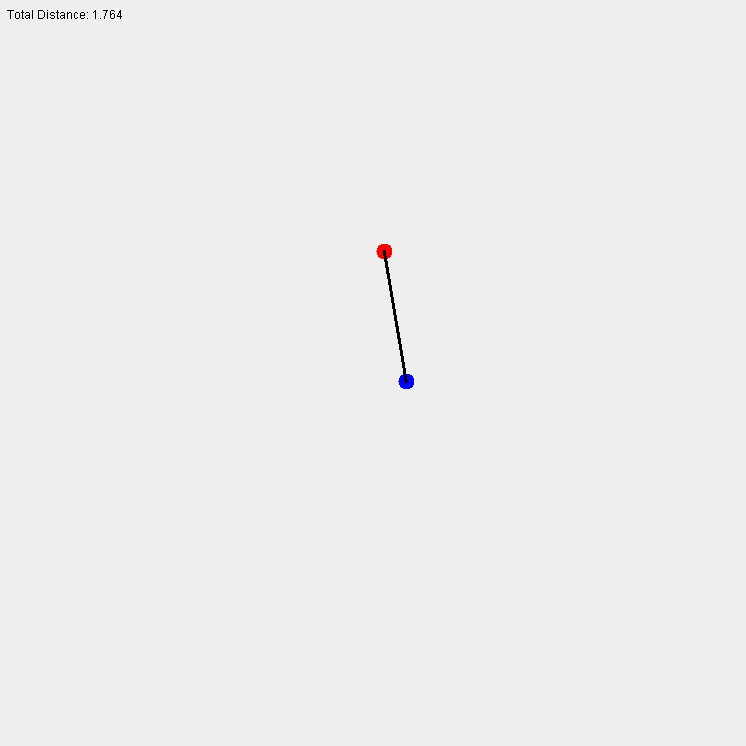
\includegraphics[width=0.4\textwidth]{./Bilder/insert_first_BAD_ex_1.PNG}
    }
    \hfil
    \subfloat[$m = 3$\label{subfig-2:m3}]{%
      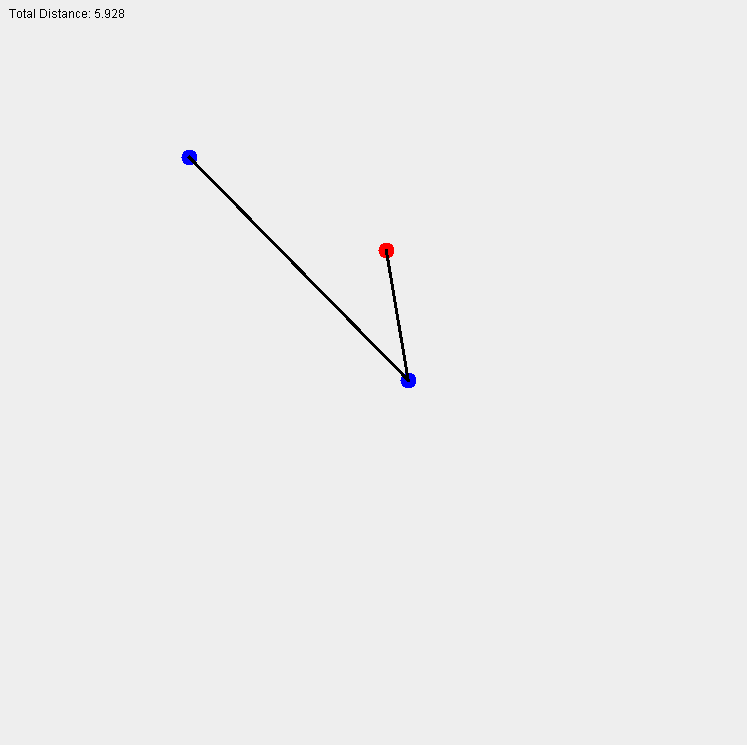
\includegraphics[width=0.4\textwidth]{./Bilder/insert_first_BAD_ex_2.PNG}
    }
    \\
    \subfloat[$m = 4$\label{subfig-3:m4}]{%
      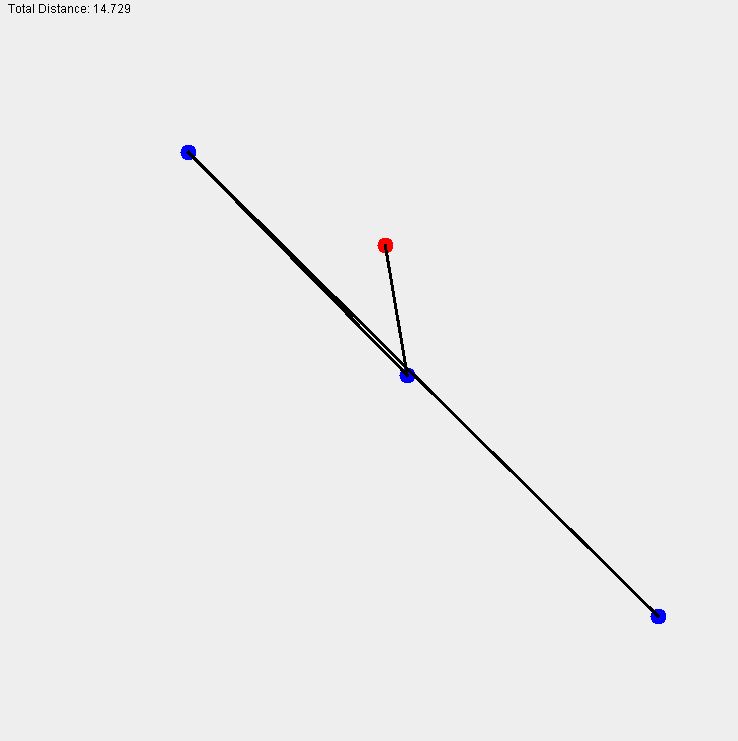
\includegraphics[width=0.4\textwidth]{./Bilder/insert_first_BAD_ex_3.PNG}
    }
    \hfil
    \subfloat[$m = 5$\label{subfig-4:m5}]{%
      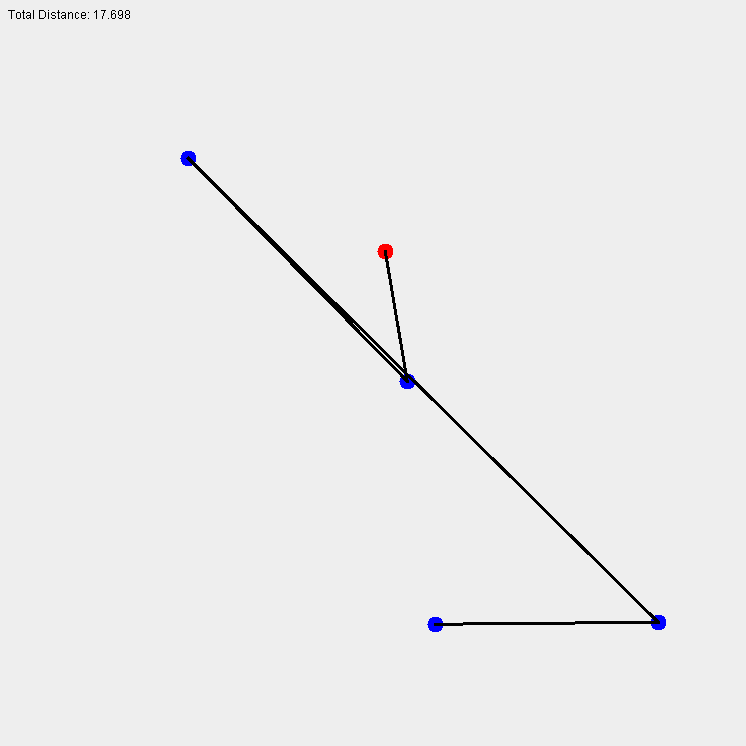
\includegraphics[width=0.4\textwidth]{./Bilder/insert_first_BAD_ex_4.PNG}
    }
    \caption{Insert-First führt zu schlechtem Ergebnis}
    \label{fig:dummy}
\end{center}

  \end{figure}

  Auf \vref{subfig-3:m4} lässt sich erkennen, dass das Einfügen des vierten Knoten $K_4$ nicht optimal geschieht. Besser für $m = 4$ wäre hier der Pfad $K_1, K_3, K_2, K_4$. 
  Dieser wird allerdings nicht das Insert-First-Verfahren gebildet, da dies eine Änderung des Graphen in \vref{subfig-2:m3} erfordern würde. 
  Dies ist allerdings nicht möglich, da $K_4$ nur zwischen bereits im Pfad des Graphen vorhandenen Knoten eingefügt werden kann.